% Options for packages loaded elsewhere
\PassOptionsToPackage{unicode}{hyperref}
\PassOptionsToPackage{hyphens}{url}
%
\documentclass[
]{article}
\usepackage{amsmath,amssymb}
\usepackage{lmodern}
\usepackage{iftex}
\ifPDFTeX
  \usepackage[T1]{fontenc}
  \usepackage[utf8]{inputenc}
  \usepackage{textcomp} % provide euro and other symbols
\else % if luatex or xetex
  \usepackage{unicode-math}
  \defaultfontfeatures{Scale=MatchLowercase}
  \defaultfontfeatures[\rmfamily]{Ligatures=TeX,Scale=1}
\fi
% Use upquote if available, for straight quotes in verbatim environments
\IfFileExists{upquote.sty}{\usepackage{upquote}}{}
\IfFileExists{microtype.sty}{% use microtype if available
  \usepackage[]{microtype}
  \UseMicrotypeSet[protrusion]{basicmath} % disable protrusion for tt fonts
}{}
\makeatletter
\@ifundefined{KOMAClassName}{% if non-KOMA class
  \IfFileExists{parskip.sty}{%
    \usepackage{parskip}
  }{% else
    \setlength{\parindent}{0pt}
    \setlength{\parskip}{6pt plus 2pt minus 1pt}}
}{% if KOMA class
  \KOMAoptions{parskip=half}}
\makeatother
\usepackage{xcolor}
\usepackage[margin=1in]{geometry}
\usepackage{color}
\usepackage{fancyvrb}
\newcommand{\VerbBar}{|}
\newcommand{\VERB}{\Verb[commandchars=\\\{\}]}
\DefineVerbatimEnvironment{Highlighting}{Verbatim}{commandchars=\\\{\}}
% Add ',fontsize=\small' for more characters per line
\usepackage{framed}
\definecolor{shadecolor}{RGB}{248,248,248}
\newenvironment{Shaded}{\begin{snugshade}}{\end{snugshade}}
\newcommand{\AlertTok}[1]{\textcolor[rgb]{0.94,0.16,0.16}{#1}}
\newcommand{\AnnotationTok}[1]{\textcolor[rgb]{0.56,0.35,0.01}{\textbf{\textit{#1}}}}
\newcommand{\AttributeTok}[1]{\textcolor[rgb]{0.77,0.63,0.00}{#1}}
\newcommand{\BaseNTok}[1]{\textcolor[rgb]{0.00,0.00,0.81}{#1}}
\newcommand{\BuiltInTok}[1]{#1}
\newcommand{\CharTok}[1]{\textcolor[rgb]{0.31,0.60,0.02}{#1}}
\newcommand{\CommentTok}[1]{\textcolor[rgb]{0.56,0.35,0.01}{\textit{#1}}}
\newcommand{\CommentVarTok}[1]{\textcolor[rgb]{0.56,0.35,0.01}{\textbf{\textit{#1}}}}
\newcommand{\ConstantTok}[1]{\textcolor[rgb]{0.00,0.00,0.00}{#1}}
\newcommand{\ControlFlowTok}[1]{\textcolor[rgb]{0.13,0.29,0.53}{\textbf{#1}}}
\newcommand{\DataTypeTok}[1]{\textcolor[rgb]{0.13,0.29,0.53}{#1}}
\newcommand{\DecValTok}[1]{\textcolor[rgb]{0.00,0.00,0.81}{#1}}
\newcommand{\DocumentationTok}[1]{\textcolor[rgb]{0.56,0.35,0.01}{\textbf{\textit{#1}}}}
\newcommand{\ErrorTok}[1]{\textcolor[rgb]{0.64,0.00,0.00}{\textbf{#1}}}
\newcommand{\ExtensionTok}[1]{#1}
\newcommand{\FloatTok}[1]{\textcolor[rgb]{0.00,0.00,0.81}{#1}}
\newcommand{\FunctionTok}[1]{\textcolor[rgb]{0.00,0.00,0.00}{#1}}
\newcommand{\ImportTok}[1]{#1}
\newcommand{\InformationTok}[1]{\textcolor[rgb]{0.56,0.35,0.01}{\textbf{\textit{#1}}}}
\newcommand{\KeywordTok}[1]{\textcolor[rgb]{0.13,0.29,0.53}{\textbf{#1}}}
\newcommand{\NormalTok}[1]{#1}
\newcommand{\OperatorTok}[1]{\textcolor[rgb]{0.81,0.36,0.00}{\textbf{#1}}}
\newcommand{\OtherTok}[1]{\textcolor[rgb]{0.56,0.35,0.01}{#1}}
\newcommand{\PreprocessorTok}[1]{\textcolor[rgb]{0.56,0.35,0.01}{\textit{#1}}}
\newcommand{\RegionMarkerTok}[1]{#1}
\newcommand{\SpecialCharTok}[1]{\textcolor[rgb]{0.00,0.00,0.00}{#1}}
\newcommand{\SpecialStringTok}[1]{\textcolor[rgb]{0.31,0.60,0.02}{#1}}
\newcommand{\StringTok}[1]{\textcolor[rgb]{0.31,0.60,0.02}{#1}}
\newcommand{\VariableTok}[1]{\textcolor[rgb]{0.00,0.00,0.00}{#1}}
\newcommand{\VerbatimStringTok}[1]{\textcolor[rgb]{0.31,0.60,0.02}{#1}}
\newcommand{\WarningTok}[1]{\textcolor[rgb]{0.56,0.35,0.01}{\textbf{\textit{#1}}}}
\usepackage{graphicx}
\makeatletter
\def\maxwidth{\ifdim\Gin@nat@width>\linewidth\linewidth\else\Gin@nat@width\fi}
\def\maxheight{\ifdim\Gin@nat@height>\textheight\textheight\else\Gin@nat@height\fi}
\makeatother
% Scale images if necessary, so that they will not overflow the page
% margins by default, and it is still possible to overwrite the defaults
% using explicit options in \includegraphics[width, height, ...]{}
\setkeys{Gin}{width=\maxwidth,height=\maxheight,keepaspectratio}
% Set default figure placement to htbp
\makeatletter
\def\fps@figure{htbp}
\makeatother
\setlength{\emergencystretch}{3em} % prevent overfull lines
\providecommand{\tightlist}{%
  \setlength{\itemsep}{0pt}\setlength{\parskip}{0pt}}
\setcounter{secnumdepth}{-\maxdimen} % remove section numbering
\ifLuaTeX
  \usepackage{selnolig}  % disable illegal ligatures
\fi
\IfFileExists{bookmark.sty}{\usepackage{bookmark}}{\usepackage{hyperref}}
\IfFileExists{xurl.sty}{\usepackage{xurl}}{} % add URL line breaks if available
\urlstyle{same} % disable monospaced font for URLs
\hypersetup{
  pdftitle={Wood's Quadratic Programming Method},
  pdfauthor={Sophie Wulfing},
  hidelinks,
  pdfcreator={LaTeX via pandoc}}

\title{Wood's Quadratic Programming Method}
\author{Sophie Wulfing}
\date{2/17/2022}

\begin{document}
\maketitle

\begin{verbatim}
##              [,1]
##  [1,]  76.5230312
##  [2,]  27.8603269
##  [3,]   2.2288262
##  [4,]   1.8573551
##  [5,]  57.5780089
##  [6,]  37.8900446
##  [7,]   1.8573551
##  [8,]   0.0000000
##  [9,]  40.4903417
## [10,]  50.8915305
## [11,]   3.3432392
## [12,]   0.0000000
## [13,]  71.6939079
## [14,]  16.7161961
## [15,]   8.1723626
## [16,]   1.1144131
## [17,] 121.0995542
## [18,]  28.9747400
## [19,]   5.5720654
## [20,]   2.2288262
## [21,] 119.9851412
## [22,]  52.0059435
## [23,]   6.6864785
## [24,]   0.7429421
## [25,]  78.7518574
## [26,]  41.6047548
## [27,]  14.4873700
## [28,]   1.1144131
## [29,] 118.8707281
## [30,]  53.4918276
## [31,]  14.4873700
## [32,]   1.1144131
## [33,] 119.9851412
## [34,]  39.0044576
## [35,]  10.7726597
## [36,]   1.1144131
## [37,]  73.5512630
## [38,]  26.3744428
## [39,]   4.4576523
## [40,]   2.2288262
\end{verbatim}

\begin{verbatim}
##       [,1] [,2] [,3] [,4] [,5] [,6] [,7] [,8]
##  [1,]   -1    0    0    0    0    0    0    0
##  [2,]    0   -1    0    0    0    0    0    0
##  [3,]    0    0   -1    0    0    0    0    0
##  [4,]    0    0    0   -1    0    0    0    0
##  [5,]    0    0    0    0   -1    0    0    0
##  [6,]    0    0    0    0    0   -1    0    0
##  [7,]    0    0    0    0    0    0   -1    0
##  [8,]    0    0    0    0    0    0    0   -1
##  [9,]    1    1    0    0    0    0    0    0
## [10,]    0    0    1    1    0    0    0    0
## [11,]    0    0    0    0    1    1    0    0
## [12,]    0    0    0    0    0    0    0    1
\end{verbatim}

\begin{verbatim}
##           [,1]      [,2]       [,3]       [,4]
## [1,] 0.6295838 0.0000000 0.00000000 26.7004983
## [2,] 0.2752164 0.3219070 0.00000000  0.0000000
## [3,] 0.0000000 0.1300588 0.39275810  0.0000000
## [4,] 0.0000000 0.0000000 0.09317825  0.3309474
\end{verbatim}

\begin{verbatim}
 [,1]    [,2] [,3] [,4]
\end{verbatim}

{[}1,{]} ``\(P_1\)'' ``0'' ``0'' ``F4'' {[}2,{]} ``G1'' ``P2'' ``0''
``0'' {[}3,{]} ``0'' ``G2'' ``P3'' ``0'' {[}4,{]} ``0'' ``0'' ``G3''
``P4'' \[\begin{bmatrix}
$P_1$&0&0&F4 \\
G1&P2&0&0 \\
0&G2&P3&0 \\
0&0&G3&P4 \\
\end{bmatrix}\]

\[\begin{bmatrix}
0.629583847097241&0&0&26.7004982678535 \\
0.275216425741737&0.321906972442815&0&0 \\
0&0.130058765403675&0.392758096317347&0 \\
0&0&0.0931782465194735&0.330947383185268 \\
\end{bmatrix}\]

\[\begin{bmatrix}
P1 = 0.63&0&0&F4 = 26.7 \\
G1 = 0.275&P2 = 0.322&0&0 \\
0&G2 = 0.13&P3 = 0.393&0 \\
0&0&G3 = 0.093&P4 = 0.331 \\
\end{bmatrix}\]

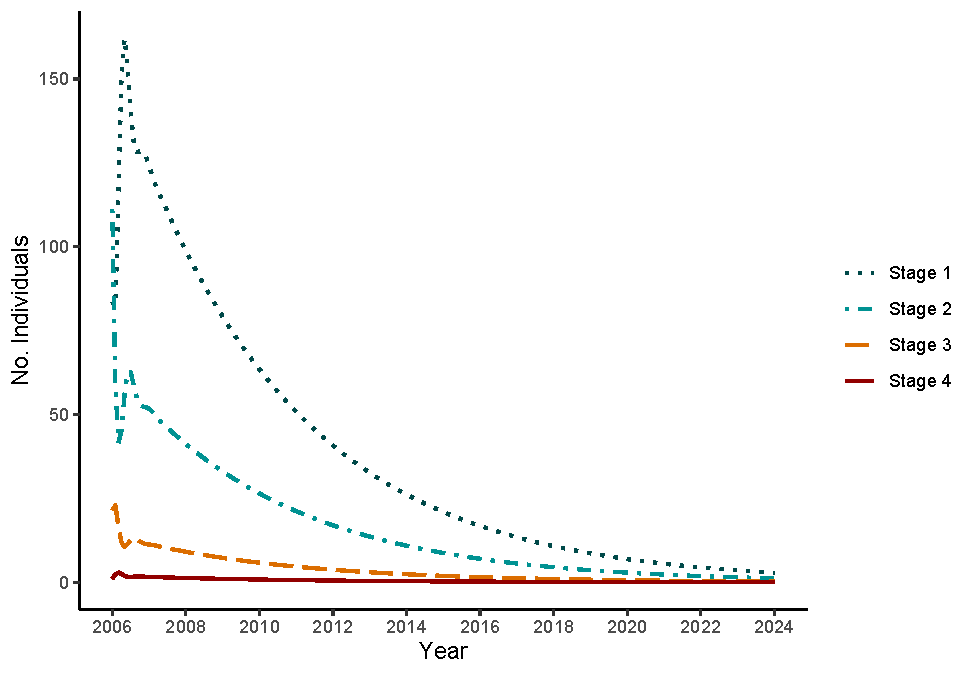
\includegraphics{Woods_Method_files/figure-latex/projection-1.pdf}

\begin{Shaded}
\begin{Highlighting}[]
\CommentTok{\#eigenvecors and vals}
\NormalTok{A\_eigen }\OtherTok{\textless{}{-}} \FunctionTok{eigen}\NormalTok{(A)}
\NormalTok{A\_eigen}
\end{Highlighting}
\end{Shaded}

\begin{verbatim}
## eigen() decomposition
## $values
## [1]  0.9817200+0.0000000i  0.4166356+0.5323073i  0.4166356-0.5323073i
## [4] -0.1397949+0.0000000i
## 
## $vectors
##                [,1]                    [,2]                    [,3]
## [1,] -0.91954608+0i -0.88561224+0.00000000i -0.88561224+0.00000000i
## [2,] -0.38355441+0i -0.07898305+0.44382834i -0.07898305-0.44382834i
## [3,] -0.08469922+0i  0.10735902+0.02411371i  0.10735902-0.02411371i
## [4,] -0.01212732+0i  0.00706315-0.01765577i  0.00706315+0.01765577i
##                [,4]
## [1,] -0.85207585+0i
## [2,]  0.50791492+0i
## [3,] -0.12404171+0i
## [4,]  0.02455269+0i
\end{verbatim}

\begin{Shaded}
\begin{Highlighting}[]
\CommentTok{\#Intrinsic Rate of Increast (r): lambda = e\^{}r}
\NormalTok{r }\OtherTok{\textless{}{-}} \FunctionTok{log}\NormalTok{(A\_eigen}\SpecialCharTok{$}\NormalTok{values[}\DecValTok{1}\NormalTok{])}
\NormalTok{r}
\end{Highlighting}
\end{Shaded}

\begin{verbatim}
## [1] -0.01844917+0i
\end{verbatim}

\begin{Shaded}
\begin{Highlighting}[]
\CommentTok{\#stable stage dist}
\NormalTok{A\_stable\_stage }\OtherTok{\textless{}{-}}\NormalTok{ A\_eigen}\SpecialCharTok{$}\NormalTok{vectors[,}\DecValTok{1}\NormalTok{]}\SpecialCharTok{/}\FunctionTok{sum}\NormalTok{(A\_eigen}\SpecialCharTok{$}\NormalTok{vectors[,}\DecValTok{1}\NormalTok{]) }
\NormalTok{A\_stable\_stage}
\end{Highlighting}
\end{Shaded}

\begin{verbatim}
## [1] 0.65685286+0i 0.27398172+0i 0.06050260+0i 0.00866282+0i
\end{verbatim}

\begin{Shaded}
\begin{Highlighting}[]
\CommentTok{\#reproductive value}
\NormalTok{A\_repro\_value }\OtherTok{\textless{}{-}} \FunctionTok{eigen}\NormalTok{(}\FunctionTok{t}\NormalTok{(A))}\SpecialCharTok{$}\NormalTok{vectors[,}\DecValTok{1}\NormalTok{]}\SpecialCharTok{/}\FunctionTok{eigen}\NormalTok{(}\FunctionTok{t}\NormalTok{(A))}\SpecialCharTok{$}\NormalTok{vectors[}\DecValTok{1}\NormalTok{,}\DecValTok{1}\NormalTok{]}
\NormalTok{A\_repro\_value}
\end{Highlighting}
\end{Shaded}

\begin{verbatim}
## [1]  1.000000+0i  1.279488+0i  6.491088+0i 41.028923+0i
\end{verbatim}

\begin{Shaded}
\begin{Highlighting}[]
\CommentTok{\#mean reproductive value{-} is the avg no offspring?}
\NormalTok{A\_repro\_value }\SpecialCharTok{\%*\%}\NormalTok{ A\_stable\_stage}
\end{Highlighting}
\end{Shaded}

\begin{verbatim}
##             [,1]
## [1,] 1.755563+0i
\end{verbatim}

\begin{Shaded}
\begin{Highlighting}[]
\CommentTok{\#. Vandermeer (1975, 1978)}

\CommentTok{\#DO KEYFIT FUNCTION:}
\DocumentationTok{\#\# Keyfitz function}
\NormalTok{keyfitz}\OtherTok{\textless{}{-}}\ControlFlowTok{function}\NormalTok{(x,y)\{ }\CommentTok{\# you provide the observed x}
\FunctionTok{sum}\NormalTok{(}\FunctionTok{abs}\NormalTok{(x}\SpecialCharTok{{-}}\NormalTok{y))}\SpecialCharTok{/}\DecValTok{2} \CommentTok{\# and stable stage dist vectors}
\NormalTok{\} }
\CommentTok{\#SEE https://cws.auburn.edu/shared/files\%3Fid=217\&filename=ConMan\_FileDownload\_MatrixPopulation.pdf}

\CommentTok{\#Good eigval and vector sources;}
\CommentTok{\#https://setosa.io/ev/eigenvectors{-}and{-}eigenvalues/}
\CommentTok{\#http://biom300.weebly.com/eigenvalues{-}and{-}eigenvectors{-}in{-}r.html}
\end{Highlighting}
\end{Shaded}

\includegraphics{Woods_Method_files/figure-latex/lifeHistory-1.pdf}

\includegraphics{Woods_Method_files/figure-latex/sensElas-1.pdf}
\includegraphics{Woods_Method_files/figure-latex/sensElas-2.pdf}

\begin{Shaded}
\begin{Highlighting}[]
\NormalTok{cols }\OtherTok{\textless{}{-}} \FunctionTok{hcl.colors}\NormalTok{(}\DecValTok{1000}\NormalTok{, }\AttributeTok{palette =} \StringTok{"Greens 3"}\NormalTok{, }\AttributeTok{alpha =} \ConstantTok{NULL}\NormalTok{, }\AttributeTok{rev =} \ConstantTok{TRUE}\NormalTok{, }\AttributeTok{fixup =} \ConstantTok{TRUE}\NormalTok{)}\CommentTok{\#, end = .85)}

\NormalTok{elas }\OtherTok{\textless{}{-}} \FunctionTok{elasticity}\NormalTok{(A)}

\ControlFlowTok{for}\NormalTok{(i }\ControlFlowTok{in} \DecValTok{1}\SpecialCharTok{:}\FunctionTok{length}\NormalTok{(A))\{}
  \ControlFlowTok{if}\NormalTok{(A[i] }\SpecialCharTok{==} \DecValTok{0}\NormalTok{)\{}
\NormalTok{    elas[i] }\OtherTok{\textless{}{-}}  \ConstantTok{NA}
\NormalTok{  \}}
\NormalTok{\}}

\FunctionTok{image2}\NormalTok{(elas, }\AttributeTok{mar=}\FunctionTok{c}\NormalTok{(}\DecValTok{1}\NormalTok{,}\FloatTok{3.5}\NormalTok{,}\DecValTok{5}\NormalTok{,}\DecValTok{1}\NormalTok{), }\AttributeTok{border=}\StringTok{"gray70"}\NormalTok{, }\AttributeTok{col =} \FunctionTok{c}\NormalTok{(}\StringTok{"white"}\NormalTok{, cols[}\DecValTok{150}\SpecialCharTok{:}\DecValTok{850}\NormalTok{]), }\AttributeTok{text.cex =} \DecValTok{2}\NormalTok{ )}
\end{Highlighting}
\end{Shaded}

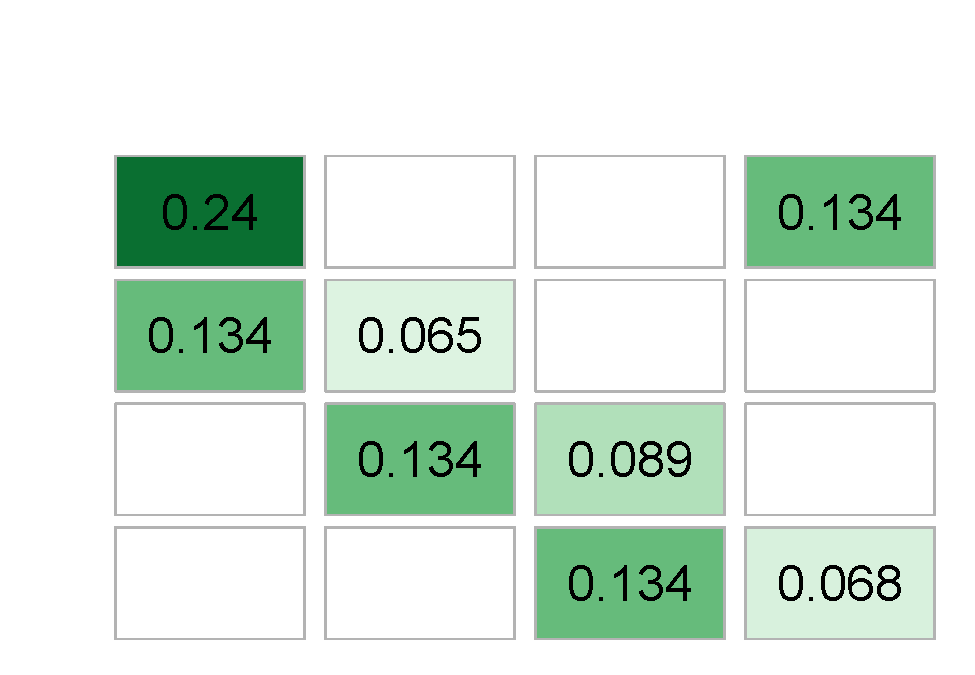
\includegraphics{Woods_Method_files/figure-latex/elasticity-1.pdf}

\begin{Shaded}
\begin{Highlighting}[]
\CommentTok{\# \# Summed elasticities for teasel.}
\CommentTok{\# \# fertility in last column, stasis P on diagonal, and growth in bottom{-}left triangle}
\CommentTok{\# c(F=sum(elas[,4]), P=sum(diag(elas)), G=sum(elas[row(elas)\textgreater{}col(elas)]))}
\CommentTok{\# }
\CommentTok{\# elas \textless{}{-} elasticity(tortoise[["med.high"]])}
\CommentTok{\# image2(elas, mar=c(1,3.5,5,1),  log=FALSE)}
\CommentTok{\#  title("Tortoise elasticity matrix", line=2.5)}
\CommentTok{\# \# Summed elasticities for tortoise (see example 9.4)}
\CommentTok{\# \# fertility in top row, stasis on diagonal, and growth on subdiagonal}
\CommentTok{\# c(F=sum(elas[1,]), P=sum(diag(elas)), G=sum(elas[row(elas)==col(elas)+1]))}

\CommentTok{\#https://rdrr.io/cran/popbio/man/elasticity.html}
\end{Highlighting}
\end{Shaded}

Possible Helpful Links:

\url{https://stackoverflow.com/questions/12349122/solving-quadratic-programming-using-r}

\url{https://stackoverflow.com/questions/55727368/how-to-minimize-a-function-in-r-with-two-constraints}

\url{https://stackoverflow.com/questions/31301694/least-square-optimization-of-matrices-in-r?rq=1}

\url{https://henrywang.nl/quadratic-programming-with-r/}

\url{https://cran.r-project.org/web/packages/quadprog/quadprog.pdf}

Also when you start doing this in markdown, here's the website for
citations:
\url{https://www.anthonyschmidt.co/post/2021-10-25-a-zotero-workflow-for-r/}

\end{document}
